%\documentclass[10pt, conference, compsocconf]{IEEEtran}
\documentclass[conference]{IEEEtran}

\usepackage{graphicx,epstopdf}
\usepackage{float}
\usepackage{wrapfig}
\usepackage{subfigure}
\usepackage{algorithmicx}
\usepackage{algpseudocode}
\usepackage{amsmath}
\usepackage{amssymb}
\usepackage{amsthm}
\usepackage{url}
\usepackage{cite}
\usepackage[T1]{fontenc} % embed fonts in pdf

\DeclareGraphicsExtensions{.pdf}
\hyphenation{op-tical net-works semi-conduc-tor}

%------------------------------------------------------------------------------
%------------------------------------------------------------------------------
%------------------------------------------------------------------------------

\begin {document}

\title {On the Acceleration of Viola-Jones Face Detection Algorithm on FPGAs}

\author
{
\IEEEauthorblockN{Curtis Bader, Peter Irgens, Theresa Le, Devansh Saxena, Cristinel Ababei}
\IEEEauthorblockA{Department of Electrical and Computer Engineering \\
Marquette University, Milwaukee WI, USA \\
Email: \{curtis.bader,peter.irgens,theresa.le,devansh.saxena,cristinel.ababei\}@marquette.edu}
}

%\IEEEoverridecommandlockouts
%\IEEEpubid{\makebox[\columnwidth]{978-1-4673-2154-9/12/\$31.00~\copyright~2012 IEEE \hfill} \hspace{\columnsep}\makebox[\columnwidth]{ }}
	      
\maketitle

%------------------------------------------------------------------------------
%------------------------------------------------------------------------------
%------------------------------------------------------------------------------

\begin {abstract}


We present an FPGA based hardware accellerator for the popular Viola-Jones face detection algorithm.
We start by first presenting a detailed discussion of the algorithm. The scope of this discussion is to understand the internal structure of the algorithm and thus identify its primary computational bottlenecks. These computational bottlenecks represent the main candidate portions for speed-up via efficient implementation and parallelization on FPGAs. 
Selected portions of the algorithm are then coded in VHDL. The VHDL implementation is verified on a DE2-115 board, which uses a Cyclone IV FPGA chip.
Experimental results are compared against simulations performed using in-house both pure C++ as well as CUDA programmed implementations of the Viola-Jones algorithm.
The FPGA accelerated version is $4\times$ faster.


\end {abstract}

\begin{IEEEkeywords}
face detection; Viola-Jones algorithm; CUDA programming; FPGA accellerator

\end{IEEEkeywords}

\IEEEpeerreviewmaketitle

%------------------------------------------------------------------------------
%------------------------------------------------------------------------------
%------------------------------------------------------------------------------


%\vspace{-2mm}
\section {Introduction}


Field programmable gate arrays (FPGAs) have been gaining a lot in popularity because the gap between their performance and power consumption, compared to specialized ASICs, has been closing in recent years.
FPGAs are currently used in virtually any application domain.


%------------------------------------------------------------------------------
%------------------------------------------------------------------------------
%------------------------------------------------------------------------------


%\vspace{-2mm}
\section {Related Work}

Here, we describe previous attempts to speed-up the Viola-Jones algorithm via various hardware accelerators.  The attempts to speed up the Viola-Jones algorithm can be categorized as follows: multithreading, GPU-based, and FPGA-based.  By far, the most popular attempt was GPU-based.  Hefenbrock et al. \cite{hefenbrock-2010} were able to realize a 15.2 FPS (frames per second) CUDA-based implementation of running the Viola-Jones algorithm on multiple windows of the image simultaneously.  Wang et al. \cite{wang-2012} used OpenCL in parallel with the Viola-Jones algorithm and minimized the time cost on both AMD and NVidia GPU platforms.  Li et al. \cite{ligpu-2012} achieved a 3.07x speedup with more than a 50\% power reduction on the Sandy Bridge processor, a processor that integrates GPU cores along with the CPU cores on the same die. Li et al. \cite{lisurf-2012} used the Sandy Bridge processor again but instead used the SURF (speeded up robust features) algorithm to detect faces and achieved a similar speed-up as before with a speed-up of 1.42 as compared to the single thread implementation on a CPU.  Oro et al. \cite{oro-2011} used NVidia GPUs and sustained a throughput of 35 FPS under 1080p resolutions.  Kong and Deng \cite{kong-2010} achieved over 20x speedup using a CPU-GPU cooperative implementation for the Viola-Jones algorithm.


%------------------------------------------------------------------------------
%------------------------------------------------------------------------------
%------------------------------------------------------------------------------


%\vspace{-2mm}
\section {Background on Viola-Jones Face Detection Algorithm}


In this section, we present a high level description of the Viola-Jones face detection algorithm. Such a description is necessary as it will help us better understand how to port some of its key tasks into FPGA based accellerators later on.
The pseudocode description of the Viola-Jones algorithm is presented in Fig.\ref{fig_vj_pseudocode}. In the following paragraphs we discuss several key ingredients that made this algorithm the first successful realtime face detection algorithm.


\begin{figure}[!htb]
\begin{center}
\scalebox{0.94}{\small
\framebox[3.53in]{
\begin{minipage}[t]{3.5in}
{\bf Algorithm}: Viola-Jones Face Detection Algorithm
\hrule
\begin{algorithmic}[1]
\State Input: original test image 
\State Output: image with face indicators as rectangles 

\For { $i \gets 1$ to number of scales in image pyramid } 
	\State Downsample image to create $image_i$
	\State Compute integral image, $image_{ii}$
	\For { $j \gets 1$ to number of shift steps of sub-window}
	
		\For { $k \gets 1$ to number of stages in cascade classifier} 
			\For { $l \gets 1$ to number of filters of stage $k$} 
				\State Filter detection sub-window
				\State Accumulate filter outputs
			\EndFor
			\If { accumulation fails per-stage threshold } 
				\State Reject sub-window as face
				\State Break this $k$ for loop
			\EndIf
		\EndFor
		
		\If { sub-window passed all per-stage threshold checks }
		  \State Accept this window as a face
		\EndIf	
	\EndFor			
\EndFor
\end{algorithmic}
\end{minipage}
}
}
\end{center}
%\vspace{-4mm}
\caption{Pseudocode of the Viola-Jones face detection algorithm.}
\label{fig_vj_pseudocode}
\end{figure}



In a face detection algorithm, we must use an accurate numerical description such that it sets human faces apart from other objects in a given image.
Such characteristics can be extracted with a committee algorithm called Adaboost \cite{adaboost-1997}. Such a committee can be created with weak classifiers to form a strong classifier by employing a voting mechanism. The Viola-Jones algorithm \cite{viola-2001} uses Haar-like {\it rectangle features} to construct classifiers. 
A Haar-like rectangle feature is a scalar product between the image and some Haar-like {\it pattern} or template.  
An example of a Haar-like pattern is shown in Fig.\ref{fig_haar_example}.a.


\begin{figure}[!htb]
\centering
\subfigure[]{
	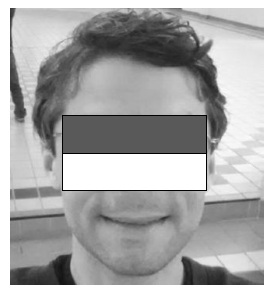
\includegraphics[scale=0.7]{fig_haar_example}
}
\subfigure[]{
	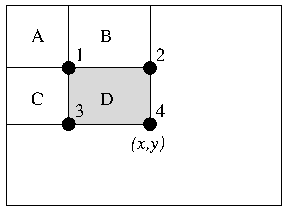
\includegraphics[scale=0.96]{fig_image_integral}
}
%\vspace{-4mm}
\caption{(a) Haar-like rectangle feature is calculated only by using the pixels inside the Haar-like pattern (i.e., black and white rectangles). This example pattern illustrates that the area covering the eyes is usually darker than the area just above the cheecks. (b) The sum of the pixels inside rectangle D can be computed with four array references on values of the integral image: $4+1-(2+3)$}
\label{fig_haar_example}
\end{figure}


A crucial element of the Viola-Jones algorithm is a technique to compute rectangle features very rapidly \cite{viola-2001,wang-2014}. This technique uses an intermediate representation for the image, the so called {\it integral image}. 
The integral image at location $(x,y)$ contains the sum of the pixels above and to the left of $(x,y)$.
Instead of summing up all the pixels inside a rectangular window, this technique mirrors the use of cumulative distribution functions.  Using the integral image any rectangular sum can be computed in four array references as shown in Fig.\ref{fig_haar_example}.b.


The Viola-Jones algorithm uses so called {\it cascade classifiers}. A cascade classifier is constructed as a sequence of stages. At each stage a list of filters are applied to the area within the sliding sub-window. An example of such a multistage filter with 25 stages is shown in Fig.\ref{fig_cascade_classifier}. Each time the sliding sub-window shifts (typically pixel by pixel, but it can be more pixels at a time to further speed things up), the new region within the sliding sub-window is processed through the cascade classifier stage-by-stage. At each stage, the rectangle feature is evaluated and the weak classifier is computed. Then, a threshold check is used to see if the region is rejected as a face candidate or if it needs to continue to be processed in the next stage.


\begin{figure}[!htb]
\centering
	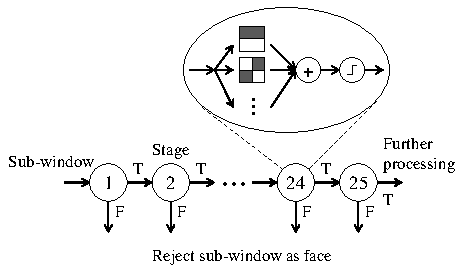
\includegraphics[scale=1.0]{fig_cascade_classifier}
%\vspace{-4mm}
\caption{Illustration of a cascade classier with 25 stages as a decision tree, where at each node a threshold check is done to decide if the sub-window is rejected as no face (False, F) or if it is passed for further processing to the next stage (True, T), which means that the sub-windows still has chances to contain a face.}
\label{fig_cascade_classifier}
\end{figure}


To be able to detect faces of different sizes, the algorithm works with a pyramid of scaled images (see Fig.\ref{fig_pyramid}). This effectively allows sweeping using the same set of Haar-like patterns different scaled versions of the initial image. Thus, sliding sub-windows will sweep each of the images from the pyramid as illustrated in Fig.\ref{fig_sliding}. 


\begin{figure}[!htb]
\centering
	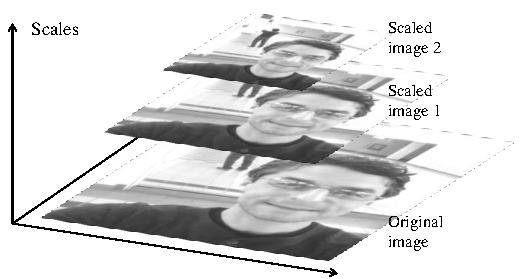
\includegraphics[scale=1.0]{fig_pyramid}
%\vspace{-4mm}
\caption{Pyramid of scaled images. The bottom image is the original image. The others are scaled images obtained via downsampling of the original image using neighboring pixels.}
\label{fig_pyramid}
\end{figure}

\begin{figure}[!htb]
\centering
	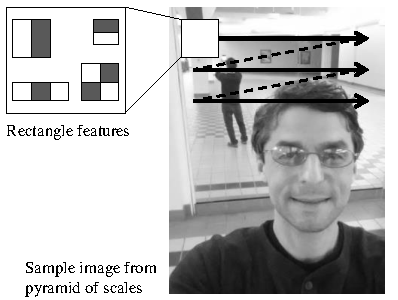
\includegraphics[scale=1.0]{fig_sliding}
%\vspace{-4mm}
\caption{Illustration of the process of sliding a sub-window. At each step during the sweeping process, the region within the sub-window has the Haar-like feature computed and processed through a cascade classifier.}
\label{fig_sliding}
\end{figure}


When the outer-most for loop in the pseudocode description from Fig.\ref{fig_vj_pseudocode} finishes its execution, the Viola-Jones algorithm would have found and marked with rectangle indicators all faces present in the original test image as well as in the scaled versions of the image. For example, Fig.\ref{fig_face_detection_example} shows the result of running the Viola-Jones algorithm on the test image from Fig.\ref{fig_sliding}.


\begin{figure}[!htb]
\centering
	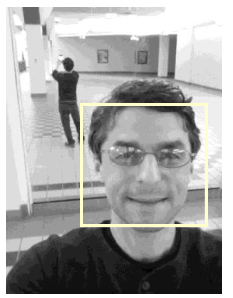
\includegraphics[scale=1.0]{fig_face_detection_example}
%\vspace{-4mm}
\caption{The output of running the Viola-Jones algorithm shows detected faces via rectangle indicators superimposed on the original test image.}
\label{fig_face_detection_example}
\end{figure}


%------------------------------------------------------------------------------
%------------------------------------------------------------------------------
%------------------------------------------------------------------------------


%\vspace{-2mm}
\section {Complexity Analysis of Viola-Jones Algorithm}


Here, we perform a computational complexity of the Viola-Jones algorithm.
We do that by using the GNU {\it gprof} tool on an in-house C++ implementation of the algorithm.



%------------------------------------------------------------------------------
%------------------------------------------------------------------------------
%------------------------------------------------------------------------------


%\vspace{-2mm}
\section {VHDL Implementation}


Once portions of the VJ algorithm have been identified as the main candidates for implementation on FPGAs, we code their functionality in VHDL.


%------------------------------------------------------------------------------
%------------------------------------------------------------------------------
%------------------------------------------------------------------------------


%\vspace{-2mm}
\section {Experimental and Simulations Results}
\label{results_section}


Here, we perform report results of the comparison between the FPGA based accelerated VJ algorithm and the C++ implementation runing on a Linux machine.

%------------------------------------------------------------------------------
%------------------------------------------------------------------------------
%------------------------------------------------------------------------------



%\vspace{-2mm}
\section {Discussion}
\label{discussion_section}


In our experiments, we found that. 


%------------------------------------------------------------------------------
%------------------------------------------------------------------------------
%------------------------------------------------------------------------------


%\vspace{-2mm}
\section {Conclusion}


We proposed an FPGA based implementation of the first face detection algorithm that was designed for real time applications. 
Our entire simulation framework is publicly available at \cite{dejazzer-software}.


%------------------------------------------------------------------------------
%------------------------------------------------------------------------------
%------------------------------------------------------------------------------


%\vspace{-1mm}
\begin {thebibliography}{100}


\bibitem {adaboost-1997}
Y. Freund and R.E. Schapire, ``A decision-theoretic generalization of on-line learning and an application to boosting," \emph{J. of Computer and System Sciences}, vol. 55, no. SS971504, pp. 119-139, 1997.

\bibitem {viola-2001}
P.A. Viola and M.J. Jones, ``Rapid object detection using a boosted cascade of simple features," \emph{IEEE Computer Society Conference on Computer Vision and Pattern Recognition (CVPR)}, 2001.
\bibitem {wang-2014}
Y.-Q. Wang, ``An analysis of the Viola-Jones face detection Algorithm," \emph{Image Processing On Line (IPOL)}, ISSN 2105-1232, 2014.

\bibitem {dejazzer-software}
%Removed temporarily for blind review.
Software downloads at MESS Lab, Marquette University, 2014. [Online]. Available: \url{http://dejazzer.com/software.html}.

\bibitem {hefenbrock-2010}
D.  Hefenbrock, J.  Oberg, N.  Thanh, R.  Kastner and S.  Baden, ``Accelerating Viola-Jones Face Detection to FPGA-Level Using GPUs," \emph{2010 18th IEEE Annual International Symposium on Field-Programmable Custom Computing Machines}, 2010.

\bibitem {wang-2012}
W. Wang, Y. Zhang, S. Yan, Y. Zhang and H. Jia, ``Parallelization and performance optimization on face detection algorithm with OpenCL: A case study," \emph{Tinshhua Sci. Technol.}, vol. 17, no. 3, pp. 287-295, 2012.

\bibitem {ligpu-2012}
E.  Li, B.  Wang, L.  Yang, Y.  Peng, Y.  Du, Y.  Zhang and Y.  Chiu, ``GPU and CPU Cooperative Accelaration for Face Detection on Modern Processors", \emph{2012 IEEE International Conference on Multimedia and Expo}, 2012.

\bibitem {lisurf-2012}
E. Li, L. Yang, B. Wang, J. Li and Y. Peng, ``SURF cascade face detection acceleration on Sandy Bridge processor", \emph{2012 IEEE Computer Society Conference on Computer Vision and Pattern Recognition Workshops}, 2012.

\bibitem {oro-2011}
D. Oro, C. Fernandez, J. Saeta, X. Martorell and J. Hernando, ``Real-time GPU-based face detection in HD video sequences", \emph{2011 IEEE International Conference on Computer Vision Workshops (ICCV Workshops)}, 2011.

\bibitem {acasandrei-2013}
L. Acasandrei and A. Barriga, ``Design methodology for face detection acceleration", \emph{IECON 2013 - 39th Annual Conference of the IEEE Industrial Electronics Society}, 2013.

\bibitem {kong-2010}
J. Kong and Y. Deng, ``GPU accelerated face detection", \emph{2010 International Conference on Intelligent Control and Information Processing}, 2010.

\bibitem {che-2010}
M. Che and Y. Chang, ``A Hardware/Software Co-design of a Face Detection Algorithm Based on FPGA", \emph{2010 International Conference on Measuring Technology and Mechatronics Automation}, 2010.

\bibitem {kumar-2014}
C. Kumar and S. Agarwal, ``A novel architecture for dynamic integral image generation for Haar-based face detection on FPGA", \emph{TENCON 2014 - 2014 IEEE Region 10 Conference}, 2014.

\end {thebibliography}

%------------------------------------------------------------------------------
%------------------------------------------------------------------------------
%------------------------------------------------------------------------------
\end{document}


